\section{RELATED WORK}

\subsection{Incremental Frequent Itemsets Mining}
The definition of an Incremental update, is to recompute outputs which depend on the incoming inputs only, without recomputing the whole data.

The challenge while performing incremental updates for frequent items mining, is a non consistent frequency order. Several algorithms such as AFPIM~\cite{koh2004efficient}, EFPIM~\cite{li2006fast} and FUFP-tree~\cite{hong2008incrementally} are keeping an updated frequency based trees, by reordering branches where frequency has changed. 

\paragraph{Canonical-Tree}
The work of~\cite{leung2005cantree} presented a Canonical Tree (CanTree) which preserves the frequency descending structure as in FP Growth mining, by relying on a predefined order, which will not affect the tree structure and correctness.

The predefined order, creates some nice properties, as described below:

\begin{enumerate}
	\item Items are arranged according to a canonical order, which is a fixed
global ordering.
	\item The ordering of items is unaffected by the changes in frequency
caused by incremental updating.
	\item The frequency of a node in the CanTree is at least as high as the sum
of frequencies of all its children.
\end{enumerate}

Since CanTree preserves same feature as the FP-Tree for mining FIS, the mining is done in the same fasion as the original FP-Growth algorithm.

An example of a CanTree is presented in \autoref{tab:table1} and \autoref{fig:CanTreeExample}

\begin{table}[h!]
  \begin{center}
    \caption{Consider the following database:}
    \label{tab:table1}
    \begin{tabular}{l|c|l} % <-- Alignments: 1st column left, 2nd middle and 3rd right, with vertical lines in between
      \textbf{} & \textbf{TID} & \textbf{Contents}\\
      \hline
      Original database (DB) & t\textsubscript{1} & {a, d, b, g, e, c}\\
       & t\textsubscript{2} & {d, f, b, a, e}\\
        & t\textsubscript{3} & {a}\\
	   & t\textsubscript{4} & {d, a, b}\\
       The first group of insertions (db1) & t\textsubscript{5} & {a, c, b}\\
        & t\textsubscript{6} & {c, b, a, e}\\
       The second group of insertions (db2) & t\textsubscript{7} & {a, b, c}\\
        & t\textsubscript{8} & {a, b, c} \\
    \end{tabular}
  \end{center}
\end{table}

\begin{figure}
  \centering
  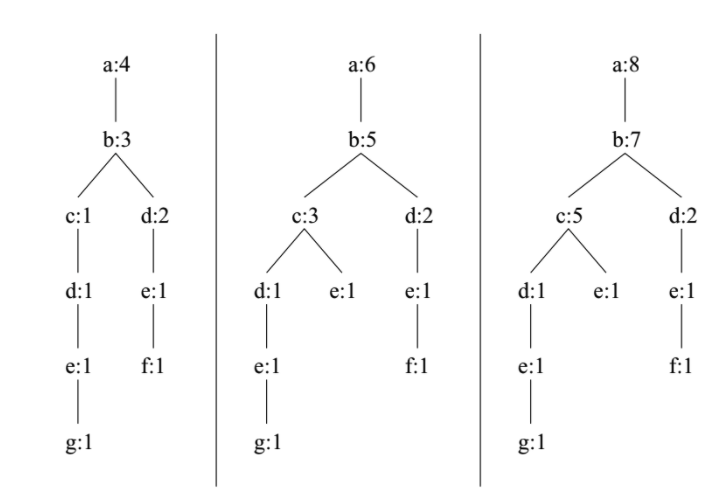
\includegraphics[width=\linewidth]{figures/CanTreeExample}
  \caption{The CanTree after each group of transactions is added}
  \label{fig:CanTreeExample}
\end{figure}

\paragraph{CP-Tree}
\label{par:cptree}
	The work of~\cite{tanbeer2009efficient} proposes an improvement to CanTree, called CompactPattern-Tree, and discusses the memory and computation limitations of CanTree for large incremental Databases. The issues are caused due to un-efficient tree structure, and CP-Tree is proposing an improvement by periodically (using a proposed guideline) updating the order of the construction literals list (l-list) and rebuilding the trees. As mention in the original article and as seen by our experiments, the CanTree and CP-Tree has a similar tree size, and the difference for our test cases was 10\% in tree sizes. However as seen in our results, using semi-frequency based order, improves the mining results by 10X and more for smaller minSupport values.


\subsection{Parallel Frequent Itemsets mining}
The difficulty in parallelizing FP-growth is to distribute iterations to parallel trees while still allowing correct mining. PFP~\cite{li2008pfp} is solving this by dividing the DB transactions to independent trees using a Group-List, where every group consists of subgroup of the original items, and redistributing iterations in the DB based on this list.
PFP~\cite{li2008pfp} has the following MapReduce stages:

\begin{steps}
\item Calculate the global frequency list F-list, by MapReduce "Work Count" manner.
\item In the second job, the the map will have the following functionality:
\begin{enumerate}
\item Sort transactions based on F-list.
\item Replace items in a transaction with the appropriate group id mapped transactions.
\end{enumerate}
	The reducer here will build the trees in a parallel manner, based on the group id of the mapping stage.
\item In the final mapping stage, every mapper will project the sub tree from a 1-item-length frequent itemset of the group, where the reducers will recursively mine those sub-trees. The parallelization in that case, can be at most equal to the number of items in the database.
\end{steps}

A more detailed description of PFP~\cite{li2008pfp} is described here \autoref{alg:pfpalg}:
\begin{algorithm}
  \caption{Highlevel description of the PFP-Growth algorithm}\label{euclid}
  \begin{algorithmic}[1]
   \label{alg:pfpalg}
    \Procedure{PFP-Growth}{}
      \State $F-List\gets$ Find global frequency list
      \State $G-list\gets$ Define a Group items
      \ForEach{$transaction$ T\textsubscript{i} $in$ DB}
        \State t\textsubscript{i}$\gets$ order by F-List frequency
		\State $G-hashed-list$\textsubscript{i} $\gets$ replace every element a\textsubscript{j} $in$ t\textsubscript{i} with Hash(g), where a\textsubscript{j}$\in g$ And $g\in G-list$
      	\ForEach{Hash(g) $\in G-hashed-list$}
      		\State $L\gets$ find its right-most location in t\textsubscript{i}
      		\State Output key'=g; value'={t\textsubscript{i}[0]…t\textsubscript{i}[L]}
      	\EndFor
      \EndFor
 	\State Group by key' = g
 	\State For each group g, build appropriate tree
 	\State For each group g, mine the generated tree.
    \EndProcedure
  \end{algorithmic}
\end{algorithm}


To better understand the distribution of transactions between groups in PFP, an example is provided in \autoref{tab:table2}. This example shows the initial state of raw transactions, sorting them frequency based, and distributing based on a G-List of single item per group -> \{C\},\{E\},\{B\},\{A\}. Last lines demonstrate the output at line 9 \autoref{alg:pfpalg} of every transaction. 

\begin{table}[h!]
  \begin{center}
    \caption{A simple example of distributed FP-Growth:}
    \label{tab:table2}
    \begin{tabular}{l|c|l} % <-- Alignments: 1st column left, 2nd middle and 3rd right, with vertical lines in between
      \textbf{} & \textbf{TID} & \textbf{Items}\\
      \hline
      Original database (DB) & t\textsubscript{1} & {A, B}\\
       & t\textsubscript{2} & {E, C}\\
        & t\textsubscript{3} & {E, A, C}\\
	   & t\textsubscript{4} & {E, C}\\
       & t\textsubscript{5} & {E, C}\\
        & t\textsubscript{6} & {B}\\
	   & t\textsubscript{7} & {A, C}\\
       & t\textsubscript{8} & {E, D, C}\\
        & t\textsubscript{9} &{E, B} \\
	   & t\textsubscript{10} & {E, B}\\
       & t\textsubscript{11} & {E, A, C}\\
        & t\textsubscript{12} & {E, C}\\
	   & t\textsubscript{13} & {B, D, C}\\
	  F-List: & A: 4, E: 9, B: 5, C: 9, D: 2 & \\
	  		\hline
	  Support=4 & Sorted transactions => [C,E,B,A] & \\
	  		\hline
	  Sorted and Filtered & t\textsubscript{1} & {B,A}\\
       & t\textsubscript{2} & {C,E}\\
        & t\textsubscript{3} & {C, E, A}\\
	   & t\textsubscript{4} & {C,E}\\
       & t\textsubscript{5} & {C,E}\\
        & t\textsubscript{6} & {B}\\
	   & t\textsubscript{7} & {C, A}\\
       & t\textsubscript{8} & {C,E}\\
        & t\textsubscript{9} &{E, B} \\
	   & t\textsubscript{10} & {E, B}\\
       & t\textsubscript{11} & {C, E, A}\\
        & t\textsubscript{12} & {C,E}\\
	   & t\textsubscript{13} & {C, B}\\
		\hline
	   G-List & \{C\},\{E\},\{B\},\{A\} &\\
		\hline
		$g\in G-List$ & Transactions & FIS\\
		\hline
		\{C\}& t\textsubscript{2},t\textsubscript{3},t\textsubscript{4},t\textsubscript{5},t\textsubscript{7},t\textsubscript{8},t\textsubscript{11},t\textsubscript{12},t\textsubscript{13}& [C]\\
		\{E\}& 		t\textsubscript{2},t\textsubscript{3},t\textsubscript{4},t\textsubscript{5},t\textsubscript{8},t\textsubscript{11},t\textsubscript{12} & [C,E]\\
		& t\textsubscript{9},t\textsubscript{10} & [E]\\
		\{B\} &t\textsubscript{1},t\textsubscript{6} & [B]\\
		&t\textsubscript{9},t\textsubscript{10} & [E,B]\\
		&t\textsubscript{13} & [C,B]\\
		\{A\} &t\textsubscript{1} & [B,A]\\
		&t\textsubscript{3},t\textsubscript{11} & [C,E,A]\\
		&t\textsubscript{7} & [C,A]\\
    \end{tabular}
  \end{center}
\end{table}

\subsection{Incremental and Parallel Frequent itemsets mining}
Combining the previous 2 sections, yields an algorithm that does not rely on frequency order and uses parallelism advantages for computations of FIS.
The drawbacks are also drawn from the 2 algorithms - large memory consumption for saving all items and recursively calculating FIS. As we will show later in the \hyperref[sec:improvements]{Improvments} section, using an approach similar to ~\cite{kohefficient} and maintaining a pre-min support, together with using a semi-freq-order as in ~\cite{tanbeer2009efficient}, will significantly improve memory and mining runtime results.



\subsection{Song et al. }
\label{sec:song}
A paper by Song et el.~\cite{song2017} proposes 2 techniques for building and mining frequent itemsets - IncBuildingPFP and IncMiningPFP. IncBuildingPFP presents a parallel model based on CanTree that supports incremental mining. This approach is similar to IPFIM and presented in \autoref{sec:ipfim}.  


\subsubsection{IncMiningPFP}
As discussed by Song et el.~\cite{song2017} (and analysed later in this article as well), using CanTree as is, will result in memory and time limitation for relatively medium datasets (>1M) even with large clusters (>100G RAM).  IncMiningPFP solves the problem of mining by constructing FP-Growth tree for shards with new incremental items. For other shards, the data is taken from cache.

IncMiningPFP consists of the following steps:
\begin{steps}
	\item Group items G-list
	\item For the base case, for each shard, save the FIS and construct full FP-Trees to save all transactions. 
	\item For every Shard:
			\begin{enumerate}
			\item calculate and save frequency list per shard group -> F-list
			\item find 1-size FIS, extract paths from FP-Trees that contain only those items and build a FP-Growth tree.
			\item Extract full FIS from FP-Growth tree and save items in shard cache.
			\end{enumerate}
	\item For every iteration dD, devide based on G-List and send to the appropriate shards (similar to same as the distribution  stage at \autoref{alg:pfpalg}).
	\item For every shard: 
				\begin{enumerate}
				\item Recalculate F-list
				\item If got new items from dD, update tree with new values
				\item If this shard has added transactions, recalculate new FIS in similar way to initial stage and update shard cache. 
				\item Return Caches FIS.
				\end{enumerate}
	\item Reduce all previous FIS, similar to PFP.
\end{steps}

In this paper, although the IPFIM and IncBuildingPFP are similar, in \autoref{sec:improvements}, we present a different technique based on the CPTree~\cite{tanbeer2009efficient} and AFPIM~\cite{koh2004efficient} approach.

Song et el.~\cite{song2017} was also tested using classic map-reduce, while here we test the performance using Spark [TODO: Add section on spark]. Spark programs iteratively run about 100 times faster than Hadoop in-memory, and 10 times faster on disk ~\cite{spark}.
